\documentclass[10pt,t]{beamer}
\usepackage[utf8]{inputenc}
\usepackage[brazil]{babel}
\usetheme{Heverlee}


%%% QUICK OPTIONS:
% (A) Math font without serifs, enable line below to make math serif:
    %\usefonttheme[onlymath]{serif}

% (B) Re-define primary colour by adjusting the RGB values
    %\definecolor{pblue}	{RGB}{206,125,66}

% (C) Title page graphic (optional) --- this is not for the background image, see \usebackgroundtemplate to change that ---
    %\titlegraphic{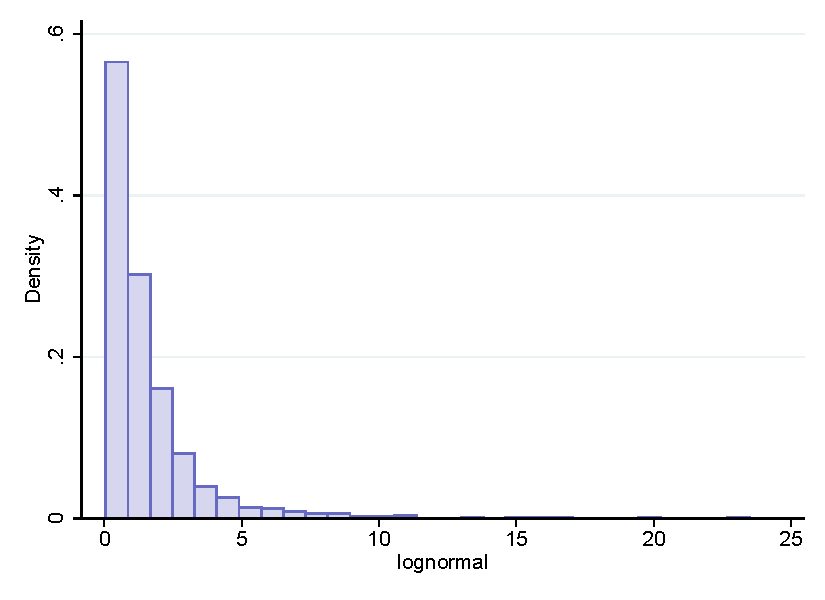
\includegraphics[height=2.7cm]{example_figure.pdf}}

% (D) Add logo to bottom right-corner (optional)
    \logo{
\includegraphics[height=0.7cm]{logo.png}\hspace{12pt}\vspace{-6pt}}      

% (E) Choose one (or none) of these lines to add footline bar on all frames
    %\setbeamertemplate{footline}[infoline]  % author, title, insitute
    %\setbeamertemplate{footline}[navigation] % dots swhowing progress
    %\setbeamertemplate{footline}[navsym] % navigation symbols

% (F) Widescreen 16:9 ratio
    %\usepackage[orientation=landscape,size=custom,width=16,height=9,scale=0.45,debug]{beamerposter} 



%%% TITLE PAGE INFO:
\title[Heverlee \LaTeX\ Beamer theme]{Painel em Python do Centro de Inteligência}
%\subtitle{\textbackslash usetheme\{Heverlee\}}
\author{Kallil de Araújo Bezerra}
\institute{Universidade Federal do Rio Grande do Norte}
\date{Outubro 2020}

% Text inside {} is used on the title page. Text inside [] is optional, and is used in footline bar (if [] is omitted then text from {} will be used in both ; if [] is specified but left empty then the footline will not show any text)




 %%
 %%  0. TITLE PAGE and TABLE OF CONTENT
 %%
\begin{document}
% Title page

{
% Change image, or delete this line to remove background image
\usebackgroundtemplate{ \parbox[b][\paperheight][b]{\paperwidth}{\centering
\includegraphics[width=\paperwidth]{Background/bg_library.jpg}}} 
 %   abudhabi      cherry      forest      river
 %   alishan       chobe       leuven      sanfancisco
 %   blueprint     columns     library     uyuni
 %   bokeh         flowers     newyork     winter

%\setbeamercolor{background canvas}{bg=lgray}  % make background light gray

\begin{frame}[plain,noframenumbering]
    \titlepage
\end{frame}
}		


% Table of contents slide
\begin{frame}{Sumário}
	\vskip 2mm
	\hfill	{\large \parbox{.95\textwidth}{\tableofcontents[hideothersubsections]}}
\end{frame}


 %%
\section{Histórico do BI e aplicações na JFRN}

\begin{frame}{Desenvolvimento do BI}\label{colorpalette}
\vspace{8pt}
Conceitos básicos de \textit{Business Intelligence}
    \begin{itemize}
        \item Termo apresentado em 1865 por Richard Millar Devens
        \item Apareceu novamente em 1958 num artigo de Hans Peter Luhn
    	\item Difundido em várias instituições - computadores menos caros
    	\item Uso da informática para suporte às \textbf{tomadas de decisões}
    	\begin{itemize}
    		\item Visualização de dados
    		\item Análise de dados
    		\item Armazenamento de dados
    	\end{itemize}
    \end{itemize}
\end{frame} 


\begin{frame}{Aplicação na JFRN}\label{colorpalette}
\vspace{8pt}
    \begin{itemize}
    	\item Usado por servidores e magistrados
    	\item Acessado através dos navegadores
    	\item Desenvolvido com Qlikview
    	\item Problemas de entendimento entre painéis
    	\item TRF5 recebe as demandas
    \end{itemize}
\end{frame} 


\begin{frame}{Portal BI}\label{colorpalette}
	\vspace{8pt}
	\begin{figure}
		\centering
		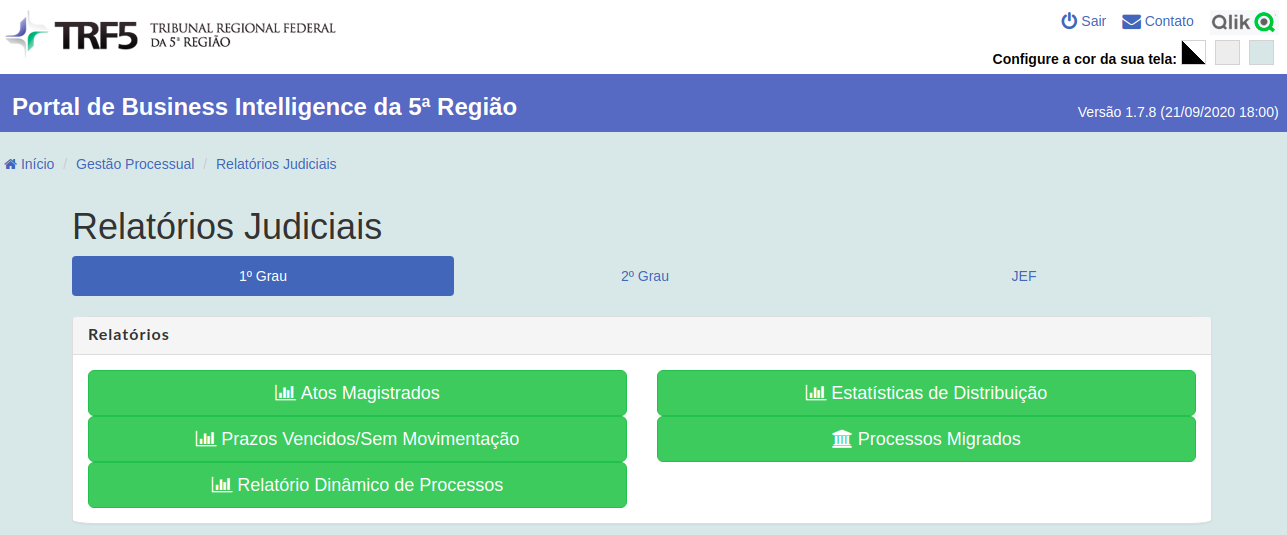
\includegraphics[scale=0.25]{./imagens/portal_bi.png}
		\caption{Portal BI do TRF5}
	\end{figure}
\end{frame} 


\begin{frame}{Ferramentas disponíveis}\label{colorpalette}
	\vspace{8pt}
	As ferramentas mais usadas:
	\begin{itemize}
		\item Qlikview
		\item PowerBI
		\item Pentaho
		\item Metabase
	\end{itemize}
\begin{figure}
	\centering
	
\includegraphics[scale=0.40]{./imagens/bi_tools.jpg}
	\caption{Ferramentas BI}
\end{figure}
\end{frame} 

\section{Construção do painel}

\begin{frame}{Escolhendo as ferramentas}\label{colorpalette}
	\vspace{8pt}
	Pontos que devem ser levados em consideração na escolha da ferramenta:
	\begin{itemize}
		\item Pago vs gratuito
		\item Pronto vs próprio
		\item Facilidade de se desenvolver
	\end{itemize}
\begin{figure}
	\centering
	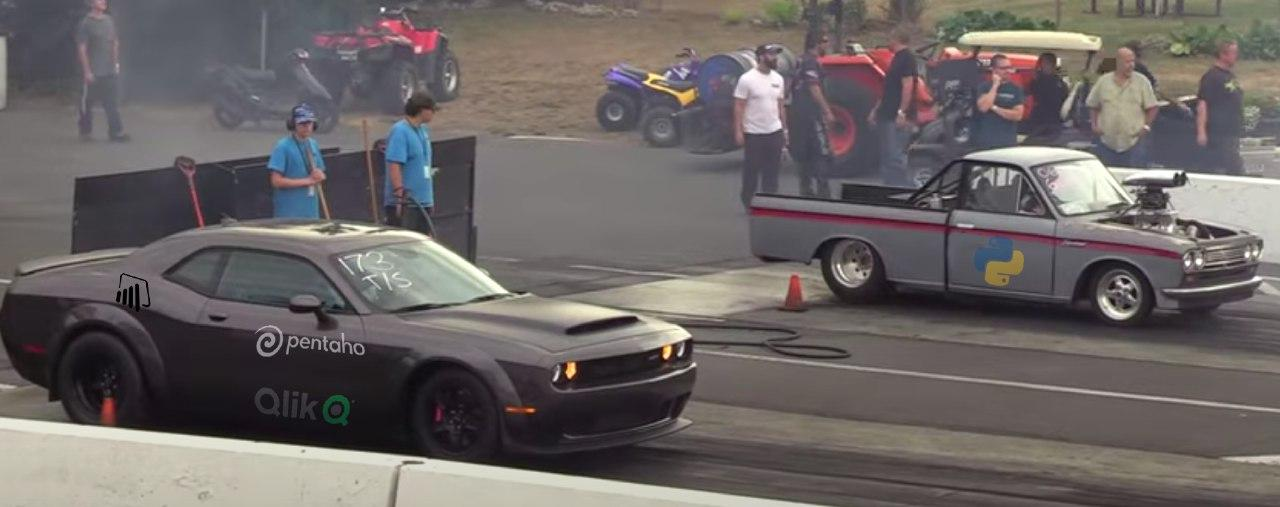
\includegraphics[scale=0.25]{./imagens/pronto_vs_construido_escolhido.jpg}
	\caption{Comprado vs construído}
\end{figure}
\end{frame} 

\begin{frame}{Prós vs Contras}
	\vspace{8pt}
	\begin{itemize}
		\item Prós: 
		\begin{itemize}
			\item Gratuito
			\item Desenvolvido \textit{in-house}
			\item Fácil de se encontrar desenvolvedores
			\item Extremamente customizável
		\end{itemize}
	    \item Contras:
	    \begin{itemize}
	    	\item Gratuito %não tem garantia
	    	\item Desenvolvido \textit{in-house} %os problemas tem que ser resolvidos localmente
	    \end{itemize}
	\end{itemize}
\end{frame}

\begin{frame}{Tecnologias usadas}
\vspace{8pt}
    \begin{itemize}
        \item Python
        \begin{itemize}
            \item Dash - visualização dos dados
            \item Numpy - análise dos dados
        \end{itemize}
        \item Qlikview - conversão dos dados para formato que possa ser lido pelo painel
    \end{itemize}
	\begin{figure}
		\centering
		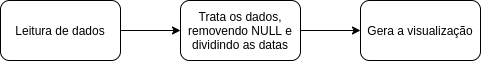
\includegraphics[scale=0.60]{./imagens/fluxo_painel.png}
		\caption{Fluxo do painel}
	\end{figure}
\end{frame}



\begin{frame}{Visualização de dados}
	\vspace{8pt}
	A importância de se ter visualização de dados que seja eficiente
\end{frame}

\begin{frame}{Análise de dados}
	\vspace{8pt}
	Falar sobre correlação e causalidade
	Lembrar de falar sobre as vendas do Xbox
    O analista de dados precisa conhecer bem os dados, ter noção do que pode ou não ser um erro é crucial para que a análise seja bem feita, e a ligação entre o time de TI e os gestores das Varas, englobando os magistrados e diretores de Vara, é importante para que as análises sejam corretas
\end{frame}

\begin{frame}{Estrutura do painel}
\vspace{8pt}
    \begin{itemize}
        \item Carregamento dos dados em formato .csv
        \item Ajuste dos dados
        \item Visualização
    \end{itemize}
\end{frame}

\section{Detecção de anomalias}

\begin{frame}{Distribuição dos dados}
	\vspace{8pt}
	\begin{itemize}
		\item Falar sobre a distribuição dos dados nas Varas
		\item Falar sobre a técnica usada
		\item Levantar alternativas
	\end{itemize}
\end{frame}


{

\setbeamercolor{background canvas}{bg=gray}
\begin{frame}[c,plain]{}
    \centering
    \textcolor{white}{Obrigado!}
\end{frame}

}














\end{document}
